
\chapter{Hidden Markov Models}

In what follows our goal is to model \textbf{time series data}. This kind of data are observed from a process evolving in time, typically at different time steps $x_1, x_2, \dots, x_N$ (i.e. assuming a discrete model of time). Since sequential data often arise through measurement of time series, there is correlation between observations at different time steps. 

These data can come from very different domains: financial data, weather forecast data, speech data, epidemiological data. 

Markov Chains are natural models for sequential data, the following is a Markov Chain of order 1:
\vspace{0.5cm}
\begin{center}
    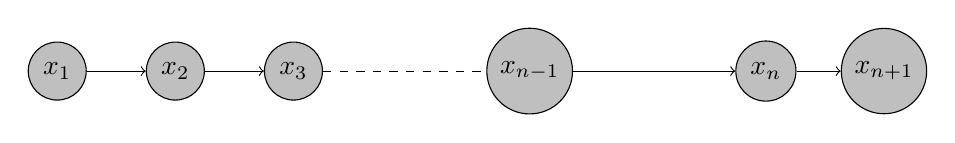
\begin{tikzpicture}
        % Nodes
        \node (x1) [circle, draw, fill=gray!50] at (-4.5, 0) {\(x_1\)};
        \node (x2) [circle, draw, fill=gray!50] at (-3, 0) {\(x_2\)};
        \node (x3) [circle, draw, fill=gray!50] at (-1.5, 0) {\(x_3\)};
        \node (xn-1) [circle, draw, fill=gray!50] at (1.5, 0) {\(x_{n-1}\)};
        \node (xn) [circle, draw, fill=gray!50] at (4.5, 0) {\(x_n\)};
        \node (xn+1) [circle, draw, fill=gray!50] at (6, 0) {\(x_{n+1}\)};
        
        % Edges
        \draw[->] (x1) -- (x2);
        \draw[->] (x2) -- (x3);
        \draw[dashed] (x3) -- (xn-1);
        \draw[->] (xn-1) -- (xn);
        \draw[->] (xn) -- (xn+1);
    
    \end{tikzpicture}
\end{center}
\vspace{0.5cm}
Since all he points (up to a certain step N) are observed, the factorization by the model is:
$$
p(x_1, x_2, \dots, x_N) = p(x_1) p(x_2 | x_1) p(x_3 | x_2) \dots p(x_N | x_{N-1})
$$

It holds that future observations are independent of all but the most recent observation:
$$
x_{n+1} \perp x_1, x_2, \dots, x_n | x_n
$$

A \textbf{time homogeneus} process is a process whose transiiton probability does not change in time, i.e. such that $p(x_1|x_{n-q}) = p(x_2|x_1)$.

These chains are not always the best model for describing sequential observations, indeed often there is a deeper dependency on the past, and first-order Markov chains suffer from too short memory. 

In these cases, we can mode to \textbf{Markov models of order k}, where the dependency of $x_n$ is on the previous $k$ steps. The following is a second order Markov Chain:
\vspace{0.5cm}
\begin{center}
    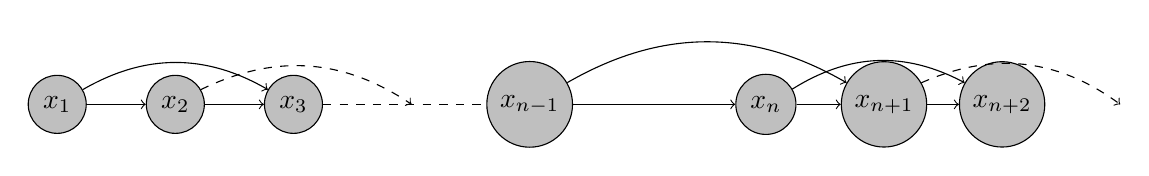
\begin{tikzpicture}
        % Nodes
        \node (x1) [circle, draw, fill=gray!50] at (-4.5, 0) {\(x_1\)};
        \node (x2) [circle, draw, fill=gray!50] at (-3, 0) {\(x_2\)};
        \node (x3) [circle, draw, fill=gray!50] at (-1.5, 0) {\(x_3\)};
        \node (xn-1) [circle, draw, fill=gray!50] at (1.5, 0) {\(x_{n-1}\)};
        \node (xn) [circle, draw, fill=gray!50] at (4.5, 0) {\(x_n\)};
        \node (xn+1) [circle, draw, fill=gray!50] at (6, 0) {\(x_{n+1}\)};
        \node (xn+2) [circle, draw, fill=gray!50] at (7.5, 0) {\(x_{n+2}\)};

        % Edges
        \draw[->] (x1) -- (x2);
        \draw[->] (x2) -- (x3);
        \draw[->, bend left] (x1) to (x3);  % Curved line from x1 to x3
        \draw[->, bend left, dashed] (x2) to (0,0);  % Curved dashed line from x2 to xn-1
        \draw[->, bend left] (xn-1) to (xn+1);  % Curved line from xn-1 to xn+1
        \draw[->, bend left] (xn) to (xn+2);  % Curved line from xn to xn+2
        \draw[->, bend left, dashed] (xn+1) to (9, 0);
        \draw[dashed] (x3) -- (xn-1);
        \draw[->] (xn-1) -- (xn);
        \draw[->] (xn) -- (xn+1);
        \draw[->] (xn+1) -- (xn+2);
    \end{tikzpicture}
\end{center}

In this case, the factorization of the model is:
$$
p(x_1, x_2, \dots, x_N) = p(x_1)p(x_2|x_1)p(x_3|x_2,x_1) \dots p(x_{n+1}|x_n, x_{n-1}) \dots
$$

And it holds that:
$$
x_{n+2} \perp x_{n-1} | x_n, x_{n+1}
$$

\textbf{Remark}: if $x_i$ are discrete, we talk about \textit{Markov chains}; if $x_i$ are continuous and $p(x_n|\dots)$ are Gaussian, we talk about \textit{autoregressive models} (of order k).

If we want to build a model for sequential data that is not limited to the Markov assumption of any order, we can rely on \textbf{state space models}, which introduce \textbf{latent variables}. In terms of graphical model, we have that latent variables from a Markov chain, and each of them corresponds to an observation:

\begin{center}
    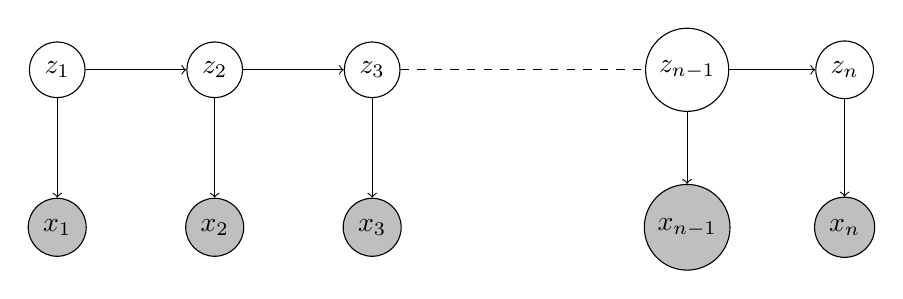
\begin{tikzpicture}
        % Nodes
        \node (x1) [circle, draw, fill=gray!50] at (-4, 0) {\(x_1\)};
        \node (x2) [circle, draw, fill=gray!50] at (-2, 0) {\(x_2\)};
        \node (x3) [circle, draw, fill=gray!50] at (0, 0) {\(x_3\)};
        \node (xn-1) [circle, draw, fill=gray!50] at (4, 0) {\(x_{n-1}\)};
        \node (xn) [circle, draw, fill=gray!50] at (6, 0) {\(x_n\)};
        \node(z1) [circle, draw] at (-4, 2) {\(z_1\)};
        \node(z2) [circle, draw] at (-2, 2) {\(z_2\)};
        \node(z3) [circle, draw] at (0, 2) {\(z_3\)};
        \node(zn-1) [circle, draw] at (4, 2) {\(z_{n-1}\)};
        \node(zn) [circle, draw] at (6, 2) {\(z_n\)};

        % Edges
        \draw[->] (z1) -- (x1);
        \draw[->] (z2) -- (x2);
        \draw[->] (z3) -- (x3);
        \draw[->] (zn-1) -- (xn-1);
        \draw[->] (zn) -- (xn);
        \draw[->] (z1) -- (z2);
        \draw[->] (z2) -- (z3);
        \draw[dashed] (z3) -- (zn-1);
        \draw[->] (zn-1) -- (zn);
    \end{tikzpicture}
\end{center}

If we consider two observations $x_i, x_j$, then $x_i \not\perp x_j|\underbar{x}$ (with $\underbar{x} = x_1, \dots, x_n$) since there is not any obserbed node in the path from $x_i$ to $x_j$.

In order to describe the space models like the one above, we need:
\begin{itemize}
    \item \textbf{transition probabilities} $p(z_n|z_{n-1})$, which describe the evolution of the latent variables. They can be arranged in a matrix A s.t. $A_{ij} = p(z_n = j|z_{n-1} = i)$;
    \item \textbf{initial distribution} $p(z_1)$, specified by a vector $\pi$ s.t. $\pi_i = p(z_1 = i)$,
    \item \textbf{emission probabilities} $p(x_n|z_n)$, parametrized by $\psi$. The emission probability for discrete $x$ is a categorical distribution, for continuous $x$ is typically a Gaussian or a mixture of Gaussians.
\end{itemize}

\begin{definitionblock}[Hidden Markov Model]
    The \textbf{Hidden Markov Model} is a specific instance of the state space model described before, in which the latent variables $z_i$ are discrete. If instead the variables $z_i$ are continuous and the transition probabilities $p(z_i|z_{i-1})$ are Gaussian, we talk about \textbf{Linear Dynamical System}.
\end{definitionblock}

Consider the parameters $\Theta = (A, \pi, \psi)$ and the variables 
$$
\underbar{x}, \underbar{z} = (x_1, \dots, x_n, z_1, \dots, z_n)
$$
then 
$$
p(\underbar{x}, \underbar{z}|\Theta) = p(z_1|\pi) \left[ \prod_{n=2}^{N}p(z_n|z_{n-1}, A) \right] \left[\prod_{n=1}^{N}p(x_n|z_n, \psi)\right]
$$

\begin{exampleblock}
    We can graphically represent the states of $\underbar{z}$ and the transition matrix as follows (note that this is not a PGM):
    \begin{center}
        \begin{tikzpicture}
            % Nodes
            \node (a) [rectangle, draw] at (0, 3) {\(a\)};
            \node (b) [rectangle, draw] at (-1.5, 0) {\(b\)};
            \node (c) [rectangle, draw] at (1.5, 0) {\(c\)};
            
            % Edges
            \draw[->] (a) -- (b);
            \draw[->] (a) -- (c);
            \draw[->] (b) -- (c);
            % arrow to themselves
            \draw[->] (a) to [out=150, in=90, looseness=8] (a);
            \draw[->] (b) to [out=150, in=90, looseness=8] (b);
            \draw[->] (c) to [out=150, in=90, looseness=8] (c);
            
        \end{tikzpicture}
    \end{center}
\end{exampleblock}